%% IEEE Conference Paper Template — compile with pdflatex + bibtex.
%% Target: 6 pages two-column IEEEtran conference.

\documentclass[conference]{IEEEtran}
\IEEEoverridecommandlockouts

\usepackage{cite}
\usepackage{amsmath,amssymb,amsfonts}
\usepackage{bbm}  % provides \mathbbm{1} — the proper indicator-function glyph
\usepackage{algorithmic}
\usepackage{graphicx}
\usepackage{textcomp}
\usepackage{xcolor}
\usepackage{booktabs}
\usepackage{balance}
\usepackage{multirow}
\usepackage{array}
\usepackage{url}
\usepackage{hyperref}
\usepackage{tikz}
\usetikzlibrary{positioning,arrows.meta,shapes.geometric,shapes.misc,calc,fit,backgrounds,patterns}
\usepackage[compact]{titlesec}

%% =====================================================================
%% UNIFORM TIGHT SPACING — applied globally so the paper compiles in 6 pages.
%% Do not add ad-hoc \vspace{-..} commands in the body; tune values here only.
%% =====================================================================

% Paragraph spacing
\setlength{\parskip}{0pt}
\setlength{\parindent}{1em}

% Float / caption spacing (figures and tables)
\setlength{\textfloatsep}{5pt plus 1pt minus 1pt}
\setlength{\intextsep}{5pt plus 1pt minus 1pt}
\setlength{\floatsep}{5pt plus 1pt minus 1pt}
\setlength{\dbltextfloatsep}{5pt plus 1pt minus 1pt}
\setlength{\dblfloatsep}{5pt plus 1pt minus 1pt}
\setlength{\abovecaptionskip}{3pt}
\setlength{\belowcaptionskip}{0pt}

% Equation / display-math spacing — pulled tight so equations sit close to surrounding text
\setlength{\abovedisplayskip}{1pt plus 1pt minus 0.5pt}
\setlength{\belowdisplayskip}{1pt plus 1pt minus 0.5pt}
\setlength{\abovedisplayshortskip}{0pt plus 1pt minus 0.5pt}
\setlength{\belowdisplayshortskip}{0pt plus 1pt minus 0.5pt}
\setlength{\jot}{1pt}
\medmuskip=3mu plus 1mu minus 2mu  % tighten medium math glue (around binary ops)
\thickmuskip=4mu plus 2mu minus 2mu  % tighten thick math glue (around relations)

% Section header spacing — uniform across \section, \subsection, \subsubsection
\titlespacing*{\section}{0pt}{5pt plus 1pt minus 1pt}{2pt plus 1pt minus 1pt}
\titlespacing*{\subsection}{0pt}{4pt plus 1pt minus 1pt}{1pt plus 1pt minus 1pt}
\titlespacing*{\subsubsection}{0pt}{3pt plus 1pt minus 1pt}{1pt plus 1pt minus 1pt}

% List spacing (enumerate / itemize)
\setlength{\topsep}{2pt plus 1pt minus 1pt}
\setlength{\partopsep}{0pt}
\setlength{\itemsep}{1pt plus 1pt minus 1pt}
\setlength{\parsep}{0pt}

\def\BibTeX{{\rm B\kern-.05em{\sc i\kern-.025em b}\kern-.08em
    T\kern-.1667em\lower.7ex\hbox{E}\kern-.125emX}}

\begin{document}

\title{\huge Enhancing Coverage and Localization in Multi-Altitude UAV Active SLAM Using Recurrent Proximal Policy Optimization}

%\author{
%\IEEEauthorblockN{Rehaan Goenka, Anjali Gupta, Manish P. Singh, and Om Jee Pandey}
%\IEEEauthorblockA{Department of Electronics Engineering, IIT (BHU), Varanasi\\
%}

\maketitle

%==================================================================
\begin{abstract}
Active Simultaneous Localization and Mapping (SLAM) for Unmanned Aerial Vehicles (UAVs) requires jointly maximizing map coverage and managing localization uncertainty while deciding at which altitude to fly. We propose a reinforcement learning framework that optimizes both objectives together. The proposed CoordConv--Long Short Term Memory (LSTM) recurrent Proximal Policy Optimization (PPO) actor-critic method is trained on a lightweight $48{\times}48{\times}4$ altitude grid environment. The method learns to vote horizontal displacement and altitude changes under a composite reward that combines per-step coverage gain, frontier direction progress, loop closure bonuses, altitude breadth incentives, and a novel covariance trace shaping term. Evaluated across three training seeds and fifty held out maps against six classical baselines and a vanilla PPO learned baseline, the proposed policy delivers higher final coverage, balanced exploration of \emph{every} altitude layer, and a roughly $2{\times}$ faster time to 50\% coverage, while matching the best baseline on localization uncertainty. The headline coverage of $\mathbf{91.90 \pm 1.72\%}$ is statistically significant against every classical baseline as well as the Vanilla PPO learned baseline, and ablations on the base recipe confirm that the altitude breadth bonus stabilizes per-altitude exploration while the loop closure reward primarily reduces localization uncertainty.
\end{abstract}

\begin{IEEEkeywords}
Active SLAM, UAV exploration, reinforcement learning, recurrent PPO, and multi-altitude planning.
\end{IEEEkeywords}

%==================================================================
\section{Introduction}

Autonomous exploration of a priori unknown three-dimensional environments is foundational for UAVs deployed in warehouses, tunnels, disaster zones, and inspection tasks \cite{qin2019autonomous, zhang2026adaptive}. The problem is doubly coupled: the agent must move to reveal new free space while localizing itself accurately enough that what it reveals can be registered into a consistent global map. This dual objective is the defining concern of active SLAM~\cite{placed2023survey, zhang2026u}.

Classical Active SLAM pipelines combine a frontier based or information theoretic controller with a backend SLAM estimator. These methods are interpretable and often effective, yet they inherit two structural limitations. First, they plan on a single two-dimensional occupancy grid, leaving altitude as a manually scheduled hyperparameter --- a mismatch with UAV stacks that operate in three-dimensional volumetric space and can exploit vertical maneuvers to see above, between, and below shelves. Second, handcrafted cost functions struggle to trade off exploration breadth, loop closure opportunity, and localization uncertainty in a single policy.

Deep Reinforcement Learning (DRL) offers an attractive alternative: given the right observation space and reward, a neural policy can learn to juggle all three concerns end-to-end. Recent work has demonstrated compelling coverage results on 2D grids~\cite{yin2025maslam,chen2024lidar,zhao2024ddpg} and on dynamic obstacle avoidance for UAVs~\cite{xu2025navrl}, but altitude aware Active SLAM policies remain underexplored, and the reward engineering required to make covariance reduction trainable alongside exploration is underdocumented.

The contributions of this work are as follows:
\begin{enumerate}
    \item \textbf{Altitude as a separate decision:} 3D exploration is decomposed into horizontal movement and altitude change. Altitude is selected via a vote with a minimum dwell rule to prevent rapid layer switching, and altitude information is fed back into the observation so a single recurrent policy handles both decisions jointly.
    \item \textbf{Position-aware network with early fusion and memory:} A CoordConv-led convolutional encoder encodes absolute map position, map features and SLAM scalars are combined via early fusion, and a recurrent layer carries context across the episode. This combination has not been applied to multi-altitude active SLAM before.
    \item \textbf{Reward shaping for localization:} A reward term $\Delta\sigma$ on the SLAM-uncertainty surrogate $\sigma_t$ (a proxy for $\mathrm{Tr}(\Sigma_t)$) densifies the rare loop-closure signal, pushing the policy toward localization-improving actions. A per-altitude breadth bonus further stabilizes layer allocation, as confirmed by ablations.
    \item \textbf{Thorough evaluation:} The policy is benchmarked against six classical baselines and a Vanilla PPO baseline across multiple seeds and held-out maps, achieving higher final coverage, balanced per-altitude exploration, and faster half-coverage time with statistically significant gains throughout.
\end{enumerate}

%==================================================================
\section{Related Work}

Prior 3D coverage and localization work splits into classical information-theoretic Active SLAM controllers and learned DRL exploration policies; we walk each thread, then surface the gap our framework closes.

\textbf{Classical active SLAM in 3D:} Placed et al.~\cite{placed2023survey} survey frontier, information-theoretic, and sampling-based exploration through 2023. Asgharivaskasi and Atanasov optimize Shannon mutual information over semantic 3D octomaps~\cite{asgharivaskasi2023semantic}, extended to Riemannian multi-robot optimization in~\cite{asgharivaskasi2025riemannian}. Ebadi et al.~\cite{ebadi2023extreme} and Azp\'urua et al.~\cite{azpurua2023subterranean} review 3D SLAM and autonomous exploration in extreme/subterranean environments. These methods are interpretable but plan in continuous 3D space with handcrafted costs --- they neither learn a policy nor decompose altitude into discrete decisions.

\textbf{Learned 3D exploration policies:} Chen et al.~\cite{chen2024lidar} present a LiDAR-based end-to-end DRL Active SLAM policy; Zhao and Hwang~\cite{zhao2024ddpg} propose an exploration--exploitation DDPG variant. Botteghi et al.~\cite{botteghi2021curiosity} use curiosity-driven rewards for indoor mapping; Yin et al.'s MA-SLAM~\cite{yin2025maslam} contributes a structured map representation for large-scale DRL exploration on ground robots. Garaffa et al.~\cite{garaffa2023survey} survey the broader literature; Wang et al.~\cite{wang2024exploration} address exploration-enhanced source search. None is altitude-aware: existing 3D-capable methods operate on full continuous 3D actions or a single planar slice.

\textbf{RL for UAVs in 3D:} NavRL~\cite{xu2025navrl} trains PPO for safe 3D UAV flight with sim-to-real transfer, but targets collision-free goal-reaching, not mapping. Kaufmann et al.~\cite{kaufmann2023racing} surpass human champions at 3D drone racing --- again navigation, not exploration. Ni et al.~\cite{ni2022recurrent} establish recurrent model-free RL as a strong POMDP baseline (motivating our LSTM backbone); Raffin et al.~\cite{raffin2021sb3} provide the Stable-Baselines3 Recurrent PPO used here.

\textbf{Positioning of our contribution:} Across these threads, no prior method jointly addresses (i) discrete altitude decisions with dwell-gated layer switches, (ii) dense covariance-trace reward shaping that turns sparse loop closures into a trainable signal, and (iii) recurrent early fusion of map and scalar state in a single learned policy --- the gap our framework closes.

%==================================================================
\section{System Model and Problem Formulation}

\subsection{System Model}

Fig.~\ref{fig:sysmodel} depicts the closed loop system for autonomous warehouse inspection. To keep RL sample efficient, we decompose the full 3D planning problem into \emph{(i)} horizontal navigation within a fixed altitude layer and \emph{(ii)} discrete altitude layer selection, and train a single recurrent policy to arbitrate between the two.

\textbf{UAV and environment:} A quadrotor carries a 2D LiDAR scanner performing a $360^\circ$ ray-sweep with $N_r\!=\!36$ uniformly-spaced beams ($N_r$: number of LiDAR beams) at the current altitude slice, plus a half-range sweep on each adjacent layer that emulates inter-layer sensor bleed and lets the agent perceive structure one altitude above and below. LiDAR is preferred over RGB/depth cameras because its range returns are robust to illumination, meaningful in feature sparse zones, and natively compatible with occupancy mapping. The warehouse is partitioned into four altitude layers $h_{\text{alt}}\!\in\!\{1,2,3,4\}\,\text{m}$ over an $X\!\times\!Y$ horizontal grid; the unknown true 3D occupancy is a binary tensor $\mathcal{M}^{\star}\!\in\!\{0,1\}^{X\times Y\times 4}$ that the agent must reconstruct within a fixed episode budget.

\textbf{Perception and observation:} Beam $i$ at step $t$ returns range $r_{i,t}$; the full sweep $\{r_{i,t}\}_{i=1}^{N_r}$ is fused by an RTAB-Map-inspired abstract SLAM proxy maintaining an occupancy estimate $\mathcal{M}_t$, a pose estimate $\hat{\xi}_t\!=\!(\hat{x}_t,\hat{y}_t,\hat{z}_t)$, and a localization-uncertainty surrogate $\sigma_t\!\in\![0,4]$ (playing the role of $\mathrm{Tr}(\Sigma_t)$). The proxy updates as $\sigma_{t+1}\!=\!\min(\sigma_t + 0.03\,\|\Delta p_t\| + 0.15\,\mathbbm{1}[\text{alt change}],\,4)$, multiplied by $0.70$ on a deterministic loop closure (agent re-enters the $r\!<\!4$ neighborhood of a stored landmark after $\geq\!40$ steps and $24$ units of travel). This SLAM state is lossy-compressed into $o_t\!=\!(M_t,v_t)$, where the map tensor $M_t\!\in\![0,1]^{5\times 48\times 48}$ stacks five altitude-aware channels (current-altitude occupancy; binary visit mask; exponentially-decaying trajectory trail; least-explored-altitude occupancy; cross-altitude mean visit mask), and the scalar vector $v_t\!\in\![0,1]^{10}$ encodes normalized uncertainty $\sigma_t/4$, frontier count, total coverage, nearest-frontier distance and direction, altitude index, current-altitude coverage, best- and worst-other-altitude coverage, and episode-step fraction $t/T_{\max}$.

\textbf{Policy and control loop:} The recurrent policy $\pi_\theta(a_t\!\mid\!o_t,h_t)$, parameterized by $\theta$ with recurrent hidden state $h_t$ (LSTM state, defined in Section~\ref{sec:arch}), emits a continuous action $a_t\!=\!(dx_t,dy_t,dz_t)\!\in\![-1,1]^3$: the first two components drive a clipped horizontal velocity command; $dz_t$ is an altitude \emph{vote} that triggers a layer change only when $|dz_t|\!>\!\tau_{\text{alt}}$, where $\tau_{\text{alt}}\!=\!0.3$ is the altitude vote threshold, and is further gated by a minimum dwell of $D\!=\!20$ steps since the last layer change, preventing the policy from thrashing the mapping backend's Z-filter.

\begin{figure*}[t]
\centering

\includegraphics[width=\textwidth,height=0.32\textwidth,keepaspectratio]{figures/system_model.png}
\caption{System model: 2D LiDAR feeds a SLAM back-end producing observation $o_t$ for the RL policy, which emits action $a_t$.}
\label{fig:sysmodel}
\end{figure*}

\subsection{Problem Formulation}

We cast the task as a POMDP $\mathcal{P}\!=\!\langle\mathcal{S},\mathcal{A},\mathcal{O},T,O_{\text{obs}},R,\gamma,T_{\max}\rangle$ over state, action, and observation spaces, with transition kernel $T$, observation kernel $O_{\text{obs}}$, reward $R$, discount $\gamma$, and horizon $T_{\max}$. The hidden state bundles the (true, unhatted) UAV pose, occupancy $\mathcal{M}_t$, and the scalar uncertainty surrogate $\sigma_t$ from Section~III-A,
\begin{equation}
s_t = \big(\, x_t, y_t, z_t,\; \mathcal{M}_t,\; \sigma_t \,\big) \in \mathcal{S},
\label{eq:state}
\end{equation}
with $\mathcal{A}\!=\![-1,1]^3$ and $\mathcal{O}\!=\![0,1]^{5\times 48\times 48}\!\times\![0,1]^{10}$ inheriting the dimensions of $a_t$ and $o_t\!=\!(M_t,v_t)$ from Section~III-A; $O_{\text{obs}}(\cdot|s_t)$ realizes the SLAM-to-observation compression, and $T(\cdot|s_t,a_t)$ is driven by UAV kinematics, SLAM updates, and loop-closure events. Heading $\psi_t$ is not stored: it is implicit in the velocity command and recomputed on demand from $(p_t-p_{t-1})$ when needed for the relative-frontier-direction scalar.

\noindent\textbf{Objective as a function of $\theta$:} Let $\pi_\theta\!:\!\mathcal{O}\!\times\!\mathcal{H}\!\to\!\Delta(\mathcal{A})$ be the recurrent policy parameterized by $\theta$, with hidden-state space $\mathcal{H}$ (the LSTM state of Section~\ref{sec:arch}) and $\Delta(\mathcal{A})$ the simplex of distributions over $\mathcal{A}$; let $\tau\!=\!(s_0,o_0,a_0,\ldots,s_{T_{\max}})$ be a trajectory it induces on $\mathcal{P}$. The \emph{expected discounted return} is
\begin{equation}
J(\theta) \,=\, \mathbb{E}_{\tau\sim\pi_\theta}\!\left[\,\sum_{t=0}^{T_{\max}-1}\gamma^{\,t}\, R(s_t,a_t)\,\right],
\label{eq:J}
\end{equation}
with $R$ the composite reward of Section~\ref{sec:reward}; $\gamma\!=\!0.995$ gives an effective horizon $1/(1-\gamma)\!\approx\!200$ steps, matched to the $T_{\max}\!=\!600$-step budget of the headline recipe ($\sim$150 steps per altitude over four layers). The target is
\begin{equation}
\theta^{\star} = \arg\max_{\theta}\; J(\theta),\qquad \pi^{\star} = \pi_{\theta^{\star}},
\label{eq:pi_star}
\end{equation}
subject to the constraint set
{\renewcommand{\arraystretch}{0.88}%
\begin{equation}
\mathcal{C}:\
\begin{cases}
a_t \in [-1,1]^3, & \forall\, t \\
a_t \sim \pi_\theta(\cdot\!\mid\!o_t,h_t), & \forall\, t \\
s_{t+1} \sim T(\cdot\!\mid\!s_t,a_t), & \forall\, t \\
o_t \sim O_{\text{obs}}(\cdot\!\mid\!s_t), & \forall\, t \\
\mathrm{alt}(t) \in \{0,1,2,3\}, & \forall\, t \\
t - \tau_{\text{last}}(t) \geq D = 20, & \text{if alt.\ change at } t \\
(x_t, y_t, z_t) \in \mathcal{F}, & \forall\, t \\
0 \leq t < T_{\max}, & T_{\max}\!\in\!\{400,600\} \\
\mathrm{Cov}(s_t)\!\geq\!0.95 \Rightarrow \text{terminate}, &
\end{cases}
\label{eq:constraints}
\end{equation}}%
where $\mathrm{alt}(t)\!=\!\lfloor z_t\rfloor\!-\!1\!\in\!\{0,1,2,3\}$ indexes the four altitude layers (recall $z_t\!\in\!\{1,2,3,4\}\,\text{m}$), $\mathcal{F}$ is collision-free configuration space, $\tau_{\text{last}}(t)$ is the most recent altitude-change timestep, and $D\!=\!20$ is the dwell from Section~III-A (set to suppress Z-filter thrashing). For ablation variants and the base/Vanilla recipes the horizon is $T_{\max}\!=\!400$; only the final headline ``MS600'' recipe uses $T_{\max}\!=\!600$.

\noindent\textbf{Coverage--localization trade-off:} Let $\mathrm{Cov}(s)$ be the fraction of true free cells in $\mathcal{M}^{\star}$ that have been observed by state $s$, and define $\mathcal{K}(\theta)\!:=\!\mathbb{E}_{\tau\sim\pi_\theta}[\mathrm{Cov}(s_{T_{\max}})]$, $\mathcal{U}(\theta)\!:=\!\mathbb{E}_{\tau\sim\pi_\theta}[\sigma_{T_{\max}}]$. Equation~\eqref{eq:J} then admits the scalarized form
\begin{equation}
J(\theta) = \underbrace{\mathcal{K}(\theta)}_{\text{max.\ cov.}} - \lambda_\sigma\underbrace{\mathcal{U}(\theta)}_{\text{min.\ unc.}} + \underbrace{\Psi(\theta)}_{\text{shaping}},
\label{eq:multiobj}
\end{equation}
with $\lambda_\sigma\!>\!0$ realized implicitly through the reward weights and $\Psi(\theta)$ collecting the per-step shaping terms (new-cell, frontier, loop-closure, breadth, absolute $\sigma$ penalty, and $\Delta\sigma$) of Section~\ref{sec:reward}.

%==================================================================
\section{Proposed Methodology}\label{sec:arch}

The policy $\pi_\theta$ is a CoordConv--LSTM actor-critic trained with Recurrent PPO~\cite{raffin2021sb3,ni2022recurrent}. It is shaped by three task-specific requirements: \emph{(i)} the filters must exploit absolute spatial position on the altitude grid; \emph{(ii)} the spatial map tensor and the scalar feature vector must be fused \emph{before} the policy commits to an action; and \emph{(iii)} partial observability demands memory across the $600$-step episode. Fig.~\ref{fig:arch} shows the complete network.

\begin{figure*}[t]
\centering
\resizebox{0.98\textwidth}{!}{
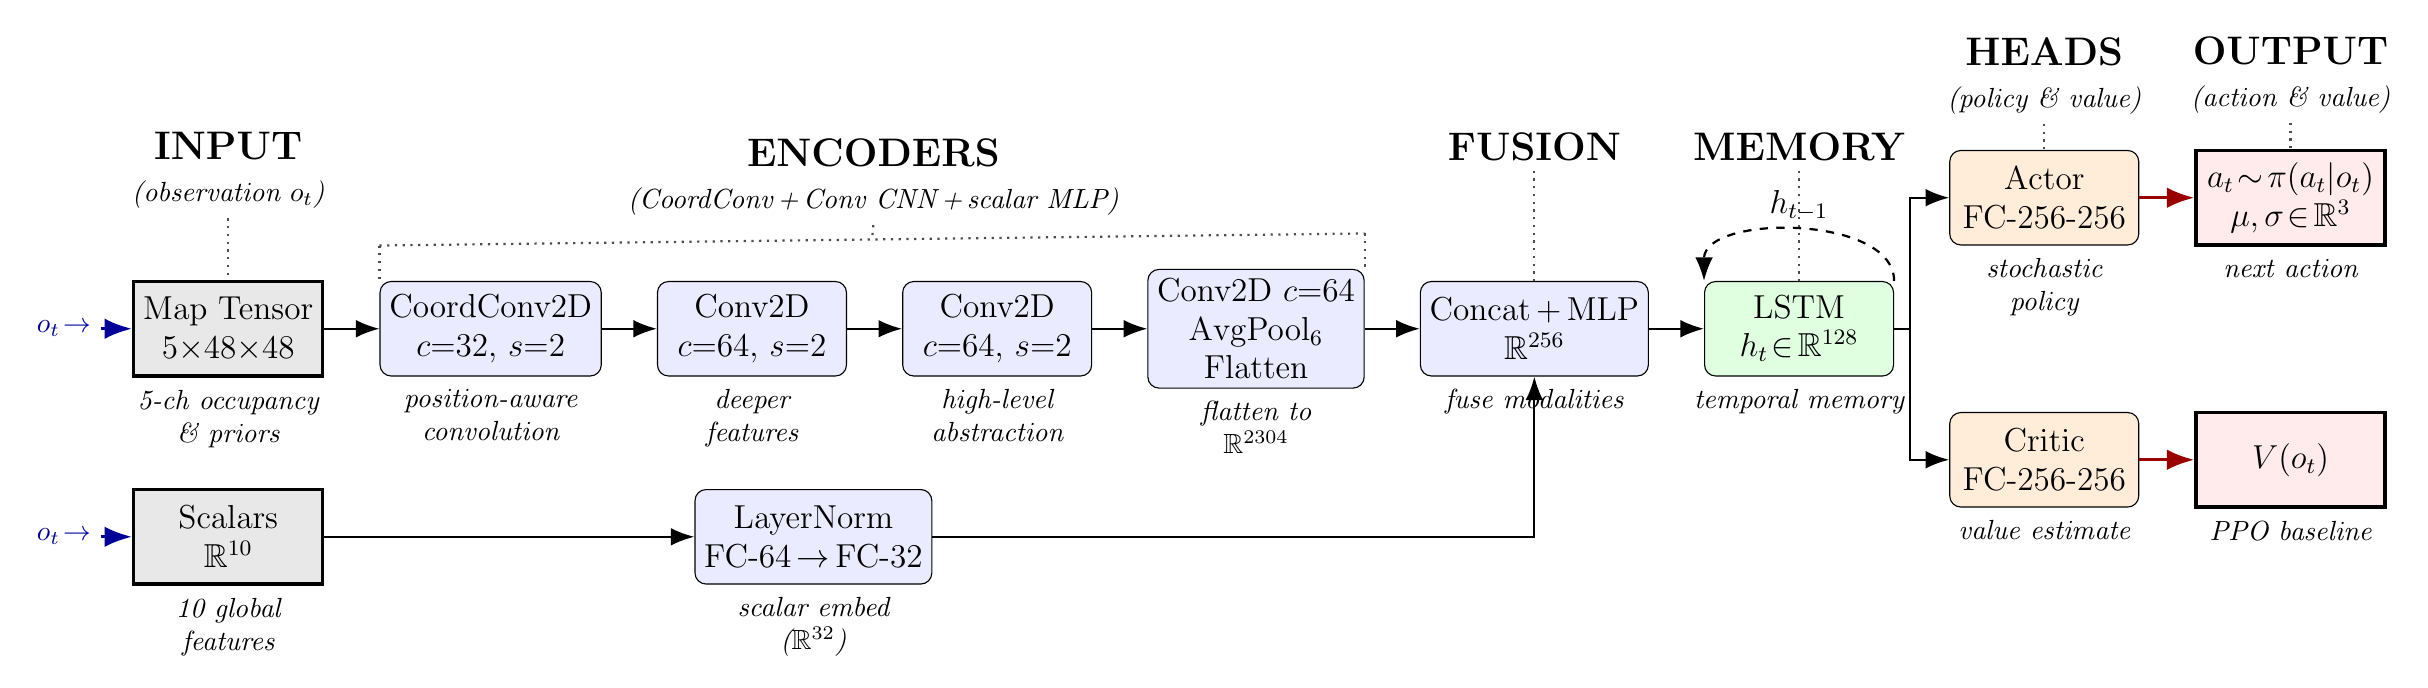
\begin{tikzpicture}[
    font=\large,
    block/.style={rectangle, draw, rounded corners, minimum height=1.2cm, minimum width=2.4cm, align=center, fill=blue!8, text=black},
    inbox/.style={rectangle, draw, very thick, minimum height=1.2cm, minimum width=2.4cm, align=center, fill=gray!18, text=black},
    outbox/.style={rectangle, draw, very thick, minimum height=1.2cm, minimum width=2.4cm, align=center, fill=red!8, text=black},
    head/.style={rectangle, draw, rounded corners, minimum height=1.2cm, minimum width=2.4cm, align=center, fill=orange!15, text=black},
    lstm/.style={rectangle, draw, rounded corners, minimum height=1.2cm, minimum width=2.4cm, align=center, fill=green!12, text=black},
    stage/.style={font=\Large\bfseries, text=black, align=center},
    sub/.style={font=\normalsize\itshape, text=black, align=center},
    ann/.style={font=\normalsize\itshape, text=black, align=center, inner sep=1pt},
    arr/.style={-{Latex[length=3mm]}, thick, text=black},
    startarr/.style={-{Latex[length=3.5mm]}, very thick, color=blue!60!black},
    endarr/.style={-{Latex[length=3.5mm]}, very thick, color=red!60!black},
    grouparr/.style={dotted, thick, color=black!70},
    node distance=0.65cm and 0.70cm
]
% ============================================================
% BLOCKS — defined first so headers can position relative to them
% ============================================================
\node[inbox] (map) {Map Tensor\\$5{\times}48{\times}48$};
\node[inbox, below=1.4cm of map] (scalars) {Scalars\\$\mathbb{R}^{10}$};

\node[left=0.4cm of map,  font=\normalsize\bfseries, color=blue!60!black] (inlab1) {$o_t\!\to$};
\node[left=0.4cm of scalars, font=\normalsize\bfseries, color=blue!60!black] (inlab2) {$o_t\!\to$};

\node[block, right=of map]   (cc1)  {CoordConv2D\\$c{=}32,\,s{=}2$};
\node[block, right=of cc1]   (cc2)  {Conv2D\\$c{=}64,\,s{=}2$};
\node[block, right=of cc2]   (cc3)  {Conv2D\\$c{=}64,\,s{=}2$};
\node[block, right=of cc3]   (fc256){Conv2D $c{=}64$\\AvgPool$_{6}$\\Flatten};

\node[block, right=4.7cm of scalars] (mlp) {LayerNorm\\FC-64\,$\to$\,FC-32};

\node[block, right=of fc256] (concat) {Concat\,+\,MLP\\$\mathbb{R}^{256}$};
\node[lstm,  right=of concat] (lstm)  {LSTM\\$h_t\!\in\!\mathbb{R}^{128}$};

\node[head,   above right=0.45cm and 0.7cm of lstm] (actor)  {Actor\\FC-256-256};
\node[head,   below right=0.45cm and 0.7cm of lstm] (critic) {Critic\\FC-256-256};

\node[outbox, right=of actor]  (action) {$a_t\!\sim\!\pi(a_t|o_t)$\\$\mu,\sigma\!\in\!\mathbb{R}^3$};
\node[outbox, right=of critic] (value)  {$V(o_t)$};

\node[ann, below=0.12cm of map]     {5-ch occupancy\\\& priors};
\node[ann, below=0.12cm of scalars] {10 global\\features};
\node[ann, below=0.12cm of cc1]     {position-aware\\convolution};
\node[ann, below=0.12cm of cc2]     {deeper\\features};
\node[ann, below=0.12cm of cc3]     {high-level\\abstraction};
\node[ann, below=0.12cm of fc256]   {flatten to\\$\mathbb{R}^{2304}$};
\node[ann, below=0.12cm of mlp]     {scalar embed\\($\mathbb{R}^{32}$)};
\node[ann, below=0.12cm of concat]  {fuse modalities};
\node[ann, below=0.12cm of lstm]    {temporal memory};
\node[ann, below=0.12cm of actor]   {stochastic\\policy};
\node[ann, below=0.12cm of critic]  {value estimate};
\node[ann, below=0.12cm of action]  {next action};
\node[ann, below=0.12cm of value]   {PPO baseline};

\node[stage, above=1.4cm of map]    (h_in)  {INPUT};
\node[sub,   below=0.02cm of h_in]  (h_in_sub)   {(observation $o_t$)};

\node[stage] (h_enc) at ($(cc1.north)!0.5!(fc256.north) + (0, 1.55)$) {ENCODERS};
\node[sub,   below=0.02cm of h_enc] (h_enc_sub) {(CoordConv\,+\,Conv CNN\,+\,scalar MLP)};

\node[stage, above=1.4cm of concat] (h_fus) {FUSION};
\node[stage, above=1.4cm of lstm]   (h_mem) {MEMORY};

\node[stage, above=0.95cm of actor] (h_head) {HEADS};
\node[sub,   below=0.02cm of h_head] (h_head_sub) {(policy \& value)};

\node[stage, above=0.95cm of action] (h_out) {OUTPUT};
\node[sub,   below=0.02cm of h_out]  (h_out_sub)  {(action \& value)};

\draw[startarr] (inlab1.east) -- (map.west);
\draw[startarr] (inlab2.east) -- (scalars.west);
\draw[arr] (map) -- (cc1);
\draw[arr] (cc1) -- (cc2);
\draw[arr] (cc2) -- (cc3);
\draw[arr] (cc3) -- (fc256);
\draw[arr] (scalars) -- (mlp);
\draw[arr] (fc256) -- (concat);
\draw[arr] (mlp.east) -- ([xshift=2mm]mlp.east) -| (concat.south);
\draw[arr] (concat) -- (lstm);
\draw[arr] (lstm.east) -- ([xshift=2mm]lstm.east) |- (actor.west);
\draw[arr] (lstm.east) -- ([xshift=2mm]lstm.east) |- (critic.west);
\draw[endarr] (actor)  -- (action);
\draw[endarr] (critic) -- (value);

\draw[arr, dashed] (lstm.north east) to[out=90, in=90, looseness=0.9]
    node[above, midway, font=\large]{$h_{t-1}$} (lstm.north west);

\draw[grouparr] (h_in_sub.south) -- (map.north);

\coordinate (encL) at ($(cc1.north west)  + (0, 0.45)$);
\coordinate (encR) at ($(fc256.north east) + (0, 0.45)$);
\coordinate (encM) at ($(encL)!0.5!(encR)$);
\draw[grouparr] (encL) -- (encR);
\draw[grouparr] (encL) -- (cc1.north west);
\draw[grouparr] (encR) -- (fc256.north east);
\draw[grouparr] (h_enc_sub.south) -- (encM);

\draw[grouparr] (h_fus.south) -- (concat.north);
\draw[grouparr] (h_mem.south) -- (lstm.north);
\draw[grouparr] (h_head_sub.south) -- (actor.north);
\draw[grouparr] (h_out_sub.south) -- (action.north);

\end{tikzpicture}
}
\caption{Proposed CoordConv--LSTM actor-critic. Map tensor is encoded by one CoordConv and three Conv2D stages; scalars by an MLP. Early-fused $256$-D embedding feeds a single-layer LSTM (hidden state $h_t$, dashed self-loop), then two $(256,256)$ heads output the action distribution and state value.}
\label{fig:arch}
\end{figure*}

\subsection{Network Design}

\textbf{Spatial map encoder:} Starting from $M_t\!\in\![0,1]^{5{\times}48{\times}48}$ --- five altitude-aware channels (current-altitude occupancy, current-altitude binary visit mask, exponentially-decaying trajectory, least-explored-altitude occupancy as a soft exploration prior, cross-altitude mean visit mask) --- one CoordConv (kernel $5$, stride $2$) and three plain Conv2D stages (two stride-$2$ followed by one stride-$1$, all kernel $3$) compute
\begin{equation}
F^{(\ell)}_t \,=\, \sigma\big(\mathrm{GN}_8\big(W^{(\ell)}\!*\!\widetilde{F}^{(\ell-1)}_t + b^{(\ell)}\big)\big),
\label{eq:coordconv}
\end{equation}
with $F^{(0)}_t\!=\!M_t$, weights $W^{(\ell)}$ and biases $b^{(\ell)}$, channel widths $32\!\to\!64\!\to\!64\!\to\!64$ across the four stages, $\sigma(\cdot)$ the ReLU, and $\mathrm{GN}_8$ a GroupNorm with $8$ groups. Only the first stage is coordinate-augmented: $\widetilde{F}^{(0)}_t$ stacks $M_t$ with two normalized coordinate maps $(i/H,\,j/W)$ over feature-map indices $(i,j)$ of height $H$ and width $W$; for $\ell\!\geq\!1$, $\widetilde{F}^{(\ell-1)}_t\!=\!F^{(\ell-1)}_t$. These coordinate channels give filters direct access to \emph{absolute} position --- a property plain convolutions lack, and one that matters in active SLAM where the same local pattern has different navigational value at a map's center vs.\ its boundary. The three strided stages collapse the $48{\times}48$ input through $24{\times}24\!\to\!12{\times}12\!\to\!6{\times}6$; the fourth (stride-$1$) stage refines features at $6{\times}6$, and an adaptive $6{\times}6$ average pool $\mathrm{AvgPool}_{6}$ (acting as identity here) followed by flattening yields the map feature
\begin{equation}
z^{\text{map}}_t \,=\, \mathrm{vec}\big(\mathrm{AvgPool}_{6}\big(F^{(4)}_t\big)\big) \,\in\, \mathbb{R}^{2304}.
\label{eq:zmap}
\end{equation}

\textbf{Scalar encoder and early fusion:} The vector $v_t\!\in\![0,1]^{10}$ (normalized covariance trace, frontier statistics, per-altitude coverages, episode progress) is layer-normalized and passed through a two-layer MLP $g_{\psi_v}$ with parameters $\psi_v$, giving $z^{\text{scl}}_t\!=\!g_{\psi_v}(v_t)\!\in\!\mathbb{R}^{32}$. The map and scalar embeddings are concatenated and re-projected by a two-layer fusion MLP $g_{\psi_f}$ with parameters $\psi_f$:
\begin{equation}
z_t \,=\, g_{\psi_f}\big([\,z^{\text{map}}_t\,;\;z^{\text{scl}}_t\,]\big) \,\in\, \mathbb{R}^{256}.
\label{eq:fuse}
\end{equation}
This \emph{early} fusion is deliberate: the policy must reason over spatial layout and scalar state jointly (``move toward this frontier \emph{because} covariance is high''), whereas late fusion would force the branches to commit to independent sub-decisions before merging.

\textbf{Recurrent backbone:} A single-layer LSTM with hidden size $128$ and parameters $\phi$ propagates context across the episode,
\begin{equation}
(h_t,\,c_t) \,=\, \mathrm{LSTM}_{\phi}\!\big(z_t;\, h_{t-1},\, c_{t-1}\big),\ \ h_t,c_t\!\in\!\mathbb{R}^{128},
\label{eq:lstm}
\end{equation}
where $h_t$ is the hidden state, $c_t$ the cell state, and $(h_0,c_0)\!=\!\mathbf{0}$ at episode start. Recurrence is indispensable: the observation is a lossy compression of history --- the trajectory channel fades old visits and $v_t$ squeezes SLAM state into ten numbers --- so $h_t$ must carry intent across multi-step strategies (e.g.\ ``commit to altitude 3 for 40 steps'') that no Markovian head could express. The hidden state is propagated through a $256$-step PPO rollout.

\textbf{Actor and critic heads:} Two independent $(256,256)$ MLPs $f_{\theta_\pi}, f_{\theta_V}$ with parameters $\theta_\pi, \theta_V$ branch from $h_t$. The actor parameterizes a diagonal Gaussian over $\mathbb{R}^3$ with mean $\mu_t\!\in\!\mathbb{R}^3$ and log-std $\log\sigma_t\!\in\!\mathbb{R}^3$,
\begin{equation}
(\mu_t,\,\log\sigma_t) = f_{\theta_\pi}(h_t),\quad a_t \sim \mathcal{N}\!\big(\mu_t,\,\mathrm{diag}(\sigma_t^2)\big),
\label{eq:actor}
\end{equation}
while the critic outputs a scalar state value $V_{\theta_V}(o_t)\!=\!f_{\theta_V}(h_t)$. Training minimizes the joint objective
\begin{equation}
\mathcal{L}(\theta_\pi,\theta_V) \,=\, \mathcal{L}^{\text{CLIP}}(\theta_\pi) \,+\, c_1\,\big(V_{\theta_V}(o_t)\!-\!\hat{R}_t\big)^2 \,-\, c_2\,\mathcal{H}[\pi_{\theta_\pi}],
\label{eq:ppo_loss}
\end{equation}
where $\mathcal{L}^{\text{CLIP}}$ is PPO's clipped-surrogate objective, $\hat{R}_t$ is the Generalized Advantage Estimation (GAE) target, $\mathcal{H}[\pi_{\theta_\pi}]$ an action-entropy bonus, and $c_1,c_2\!>\!0$ are scalar weighting coefficients~\cite{raffin2021sb3}. Separate actor/critic parameters let the critic fit the higher-frequency value signal without destabilizing the actor.

\subsection{Reward Design}\label{sec:reward}

The per-step reward $r_t$ is the weighted sum of fifteen components (Table~\ref{tab:reward}), with terminal bonuses on episode end. Three design decisions are worth highlighting.

\emph{Exploration versus localization:} The terms $\Delta n_{\text{cell}}$ and $\Delta d_{\text{front}}$ reward exploration directly. Localization is shaped by two terms with separate roles: an \emph{absolute} per-step penalty proportional to $\sigma_t/4$, and a \emph{delta} term $\Delta\sigma$ that fires whenever the surrogate uncertainty changes between steps. The delta term --- our contribution --- turns the otherwise sparse loop-closure event (which multiplicatively cuts $\sigma$ by $0.70$) into a dense per-step signal: any motion that increases $\sigma$ is mildly punished, and any loop closure produces a large negative $\Delta\sigma$ that the agent learns to seek. Its small weight ($-0.8$) keeps it from dominating the sparser exploration terms while still biasing toward uncertainty-reducing actions.

\emph{Altitude breadth:} The pair $(\mathbbm{1}[\text{new altitude}],\,\mathbbm{1}[\text{breadth}])$ converts an otherwise single-altitude planner into a multi-altitude one. The new-altitude bonus ($+25$) is paid once the first time the agent visits each layer in an episode; the breadth bonus ($+60$) is paid \emph{per altitude}, the first time \emph{that} altitude reaches $40\%$ coverage --- so the per-episode breadth payout is bounded by $4\!\times\!60\!=\!240$ and is back-loaded onto the layers the agent neglects. Removing the breadth bonus from the base recipe drops coverage by $1.0$ point and \emph{triples} the cross-seed variance on the boundary altitudes Alt0/Alt3 (Section~\ref{sec:results}).

\emph{Stagnation and terminal shaping:} A stagnation penalty ($-15$, fired when the per-altitude coverage gain is $<\!2\%$ over a $25$-step window) and the terminal $\sigma$ penalty ($-120\!\cdot\!\sigma_T/4$) prevent convergence on comfortable local minima (e.g.\ circling a single region at $70\%$ coverage). The terminal coverage bonus is itself \emph{breadth-weighted}: $+300\!\cdot\!\mathrm{Cov}\!\cdot\!(0.5+0.5\,\rho)$ where $\rho$ is the fraction of altitudes that crossed the $40\%$ breadth threshold during the episode, so terminal credit is halved if the agent ignores any layer.

\begin{table}[t]
\caption{Reward components ($\mathbbm{1}[\cdot]$: indicator). $\Delta\sigma$ is our contribution (MS600 only); Vanilla PPO keeps only $\Delta n_{\text{cell}}$, per-step, and collision.}
\label{tab:reward}
\centering
\footnotesize
\setlength{\tabcolsep}{3pt}
\begin{tabular}{@{}l r p{4.6cm}@{}}
\toprule
Term & Wt. & Semantics \\
\midrule
$\Delta n_{\text{cell}}$ & $+1.0$ & New cells observed this step \\
$\Delta d_{\text{front}}$ & $+2.0$ & Progress to nearest frontier (clipped $|\Delta|\!\leq\!3$) \\
$\mathbbm{1}[\text{coll.}]$ & $-1.0$ & Hit an occupied cell \\
per-step & $-0.05$ & Implicit budget pressure \\
revisit & $-0.15$ & Mean visited-mask in $7{\times}7$ window \\
$\mathbbm{1}[\text{new alt}]$ & $+25.0$ & First visit to a new altitude \\
$\mathbbm{1}[\text{alt sw}]$ & $-3.0$ & Cost of any altitude change \\
$\mathbbm{1}[\text{alt sw bad}]$ & $-2.0$ & Switched to a \emph{more}-explored layer \\
$\mathbbm{1}[\text{least-expl.}]$ & $+0.5$ & While at the least-explored layer \\
$\mathbbm{1}[\text{stag.}]$ & $-15.0$ & $25$ steps with $<\!2\%$ per-alt cov.\ gain \\
$\mathbbm{1}[\text{cov}\!\geq\!0.4]$ & $+30.0$ & One-time global $40\%$-coverage bonus \\
$\mathbbm{1}[\text{LC}]$ & $+25.0$ & Loop-closure event this step \\
$\mathbbm{1}[\text{breadth}_a]$ & $+60.0$ & First time alt.\ $a$ crosses $40\%$ (up to $4\!\times$) \\
$\sigma_t/4$ & $-0.8$ & Absolute uncertainty level penalty \\
$\Delta\sigma$ & $-0.8$ & Step-wise uncertainty change (\emph{ours}) \\
\midrule
Terminal cov.\ & $+300$ & $\times\,\mathrm{Cov}\!\cdot\!(0.5+0.5\rho)$; $\rho$=frac.\ of alts past $40\%$ \\
Terminal $\sigma$ & $-120$ & $\times\,\sigma_T/4$ at episode end \\
\bottomrule
\end{tabular}
\end{table}

%==================================================================
\section{Performance Evaluation}

\subsection{Experimental Conditions}

\subsubsection{Training Configuration}
Three independent seeds $\{42,100,200\}$ share an identical Recurrent-PPO setup: linear learning-rate schedule $3{\times}10^{-4}\!\to\!10^{-5}$, entropy coefficient $0.02\!\to\!0.002$, $4$ parallel envs, $n_{\text{steps}}{=}256$, batch $128$, $n_{\text{epochs}}{=}5$, $\gamma{=}0.995$, GAE $\lambda{=}0.97$, clip $0.2$, max-grad-norm $0.5$, with reward-only normalization (\texttt{VecNormalize}, $\texttt{norm\_obs}\!=\!\text{False}$, $\texttt{norm\_reward}\!=\!\text{True}$, clip $15$). Each seed trains for $800{,}000$ steps on a single NVIDIA GPU with checkpoints every $60{,}000$ steps, under a three-phase difficulty curriculum that starts at \texttt{easy}, switches to \texttt{medium} at $120{,}000$ steps, and to \texttt{hard} at $300{,}000$ steps; thereafter map difficulty is held at \texttt{hard}.

\subsubsection{Checkpoint Selection}
We select the earliest checkpoint that simultaneously (i) exceeds the strongest classical baseline (Greedy Information Gain) by at least $3$ percentage points of coverage, (ii) achieves $\sigma_T$ no greater than $0.80\!\times\!$ Greedy's, and (iii) keeps every per-altitude coverage above $25\%$. For the MS600 recipe this rule is satisfied earliest at step $180{,}000$ on every seed, and that checkpoint is fixed for all downstream evaluation. If no checkpoint satisfies all three conditions on a given seed, the script falls back to the checkpoint maximizing the composite score $\mathrm{Cov}+0.5\!\cdot\!\min_a\mathrm{Cov}_a-0.05\!\cdot\!\sigma_T$.

\subsubsection{Baselines and Evaluation Protocol}
Six classical non-learned baselines serve as comparators --- Random Walk, Nearest Frontier, Spiral, Potential Field, Greedy Information Gain~\cite{placed2023survey}, and an RRT-style frontier explorer in the spirit of Umari and Mukhopadhyay~\cite{placed2023survey}. A \emph{Vanilla PPO} learned baseline shares our network, hyperparameters, and curriculum, but disables every shaping reward except $\Delta n_{\text{cell}}$, the per-step cost, and the collision penalty (i.e.\ no breadth bonus, loop-closure bonus, frontier-direction term, revisit penalty, altitude-bonus suite, stagnation penalty, $\sigma$ penalties, or terminal bonuses). Every method is evaluated on the same $50$ held-out map seeds (\texttt{LIGHTWEIGHT\_EVAL\_SEEDS}, range $200{-}249$) with identical initial conditions; RL variants are rolled out per training seed ($n\!=\!150$ episodes total). All evaluation runs use the recipe-matched horizon ($T_{\max}\!=\!600$ for MS600, $T_{\max}\!=\!400$ otherwise), and significance is assessed via Wilcoxon signed-rank tests with Cliff's $\delta$ as the effect size.

\subsection{Results}\label{sec:results}

\subsubsection{Main Comparison}
Table~\ref{tab:main} reports all twelve methods (six classical baselines, Vanilla PPO, three learned-recipe variants, and two ablations). Our headline recipe reaches $91.90\!\pm\!1.72\%$ coverage --- a $9.17$-point absolute gain over the best classical baseline (Greedy Information Gain at $82.73\%$) and $5.03$ points over Vanilla PPO. The per-altitude breakdown shows the breadth-reward effect: our policy exceeds $85\%$ on \emph{every} altitude, while Greedy Info Gain collapses to $69.93\%$ on Alt3 and RRT Explorer to $9.48\%$.

\begin{table*}[t]
\caption{Held-out evaluation (50 maps/seed). RL: mean $\pm$ std over 3 seeds. Best learned in \textbf{bold}, best classical in \textit{italics}. Headline MS600 uses $T_{\max}\!=\!600$; all other variants and ablations use $T_{\max}\!=\!400$ on the base recipe.}
\label{tab:main}
\centering
\resizebox{\textwidth}{!}{%
\begin{tabular}{lrrrrrrrr}
\toprule
Method & Cov.\,(\%) & $\text{Tr}(\Sigma)$ & Alt0\,(\%) & Alt1\,(\%) & Alt2\,(\%) & Alt3\,(\%) & LoopCl. & AltChg \\
\midrule
Random Walk & 55.16 & 3.72 & 50.11 & 61.13 & 59.39 & 49.92 & 5.96 & 17.00 \\
Nearest Frontier & 52.53 & 3.63 & 50.67 & 61.92 & 56.45 & 41.31 & 0.00 & 3.42 \\
Spiral & 27.94 & 2.41 & 26.23 & 28.66 & 28.49 & 28.27 & 10.40 & 2.84 \\
Potential Field & 36.26 & 2.23 & 42.58 & 44.55 & 32.14 & 26.41 & 0.72 & 1.62 \\
\textit{Greedy Info Gain} & \textit{82.73} & 3.76 & 87.01 & 90.67 & 83.90 & 69.93 & 0.36 & 3.30 \\
RRT Explorer & 39.17 & 3.50 & 58.92 & 60.74 & 29.50 & 9.48 & 0.28 & 1.08 \\
\midrule
Vanilla PPO ($n{=}3$) & 86.87 $\pm$ 1.19 & 3.78 $\pm$ 0.06 & 77.67 $\pm$ 3.10 & 92.79 $\pm$ 1.30 & 93.15 $\pm$ 0.97 & 83.52 $\pm$ 1.37 & 3.35 $\pm$ 0.34 & 16.23 $\pm$ 0.23 \\
Ours --- base recipe ($n{=}3$) & 87.56 $\pm$ 2.45 & 3.71 $\pm$ 0.07 & 85.26 $\pm$ 4.97 & 94.78 $\pm$ 2.83 & 93.26 $\pm$ 2.76 & 77.12 $\pm$ 4.83 & 3.51 $\pm$ 0.06 & 16.19 $\pm$ 0.31 \\
Ours $+\Delta\sigma$ ($n{=}3$) & 88.69 $\pm$ 0.84 & 3.74 $\pm$ 0.06 & 77.47 $\pm$ 2.96 & 93.85 $\pm$ 1.13 & 95.20 $\pm$ 1.20 & 87.69 $\pm$ 2.30 & 3.39 $\pm$ 0.31 & 16.11 $\pm$ 0.24 \\
\textbf{Ours $+\Delta\sigma$ + MS600 ($n{=}3$)} & \textbf{91.90} $\pm$ \textbf{1.72} & \textbf{3.73} $\pm$ \textbf{0.11} & \textbf{88.11} $\pm$ \textbf{1.35} & \textbf{96.85} $\pm$ \textbf{0.92} & \textbf{95.79} $\pm$ \textbf{1.67} & \textbf{86.81} $\pm$ \textbf{2.91} & \textbf{7.49} $\pm$ \textbf{1.17} & \textbf{22.95} $\pm$ \textbf{1.14} \\
\midrule
Ablation: no LoopClosure reward & 89.41 $\pm$ 2.31 & 3.82 $\pm$ 0.04 & 80.84 $\pm$ 5.27 & 94.41 $\pm$ 2.78 & 95.12 $\pm$ 1.35 & 86.95 $\pm$ 1.30 & 3.49 $\pm$ 0.89 & 15.95 $\pm$ 0.80 \\
Ablation: no BreadthBonus & 86.54 $\pm$ 1.49 & 3.73 $\pm$ 0.05 & 79.46 $\pm$ 9.85 & 91.97 $\pm$ 4.33 & 92.98 $\pm$ 0.57 & 81.54 $\pm$ 9.38 & 3.48 $\pm$ 0.55 & 15.61 $\pm$ 1.24 \\
\bottomrule
\end{tabular}%
}
\end{table*}

\subsubsection{Statistical Analysis}
Table~\ref{tab:stat} pools Wilcoxon signed-rank tests of the headline MS600 policy across seeds ($n{=}150$). Our method rejects the null at $p\!<\!10^{-13}$ with $\delta\!>\!0.97$ (``large'' by Cliff's convention) against every non-learned baseline except Greedy Information Gain. The gap against Greedy Information Gain ($p\!=\!8.1{\times}10^{-14}$, $\delta\!=\!{+}0.534$) is now itself a large effect; the gap against Vanilla PPO is $p\!=\!7.4{\times}10^{-11}$ with $\delta\!=\!{+}0.486$ (large), quantifying the reward design's contribution over bare RL with identical architecture and curriculum.

\begin{table}[t]
\caption{One-sided Wilcoxon tests on coverage, MS600 vs.\ each baseline, pooled $n{=}150$. *\,$p\!<\!0.05$, **\,$p\!<\!0.01$, ***\,$p\!<\!0.001$.}
\label{tab:stat}
\centering
\small
\begin{tabular}{lrrr}
\toprule
Comparison & $p$-value & Cliff's $\delta$ & Effect \\
\midrule
Ours vs.\ Random Walk & $1.2{\times}10^{-26}$*** & $+0.990$ & large \\
Ours vs.\ Nearest Frontier & $1.4{\times}10^{-26}$*** & $+0.979$ & large \\
Ours vs.\ Spiral & $1.2{\times}10^{-26}$*** & $+1.000$ & large \\
Ours vs.\ Potential Field & $1.2{\times}10^{-26}$*** & $+0.974$ & large \\
Ours vs.\ Greedy Info Gain & $8.1{\times}10^{-14}$*** & $+0.534$ & large \\
Ours vs.\ RRT Explorer & $1.2{\times}10^{-26}$*** & $+0.997$ & large \\
Ours vs.\ Vanilla PPO & $7.4{\times}10^{-11}$*** & $+0.486$ & large \\
\bottomrule
\end{tabular}
\end{table}

\subsubsection{Training Dynamics}

\begin{figure}[t]
\centering

\includegraphics[width=\columnwidth]{figures/training_curve_coverage.png}
\caption{Coverage vs.\ training steps (mean $\pm$ std, 3 seeds). Dashed: Greedy Info Gain reference.}
\label{fig:tc-cov}
\end{figure}

\begin{figure}[t]
\centering

\includegraphics[width=\columnwidth]{figures/training_curve_per_altitude.png}
\caption{Per-altitude learning curves (solid: RL; dotted: Greedy final altitude coverage).}
\label{fig:tc-alt}
\end{figure}

Fig.~\ref{fig:tc-cov} shows that training coverage rises monotonically and exceeds the Greedy baseline by step $120{,}000$. Fig.~\ref{fig:tc-alt} reveals the multi-altitude strategy: the policy saturates the middle layers (Alt1, Alt2, where shelf content is densest) first, then brings the boundary layers (Alt0, Alt3) above $85\%$ --- a regime no classical baseline reaches.

\subsubsection{Intra-Episode Dynamics}

\begin{figure}[t]
\centering

\includegraphics[width=\columnwidth]{figures/timeseries_coverage.png}
\caption{Intra-episode coverage vs.\ step (mean $\pm$ std, 50 held-out episodes). RL reaches $50\%$ at step $\sim\!180$, $\sim\!2{\times}$ faster than Greedy.}
\label{fig:ts-cov}
\end{figure}

Fig.~\ref{fig:ts-cov} shows per-step coverage across 50 evaluation episodes. The RL policy is both more thorough (higher final coverage) and faster per unit time: the $50\%$-coverage milestone is reached at step $\sim\!180$ (RL) vs.\ $\sim\!370$ (Greedy) vs.\ $\sim\!580$ (Nearest Frontier).

\subsubsection{Ablation Analysis}
Two ablations are run on the \emph{base} recipe ($T_{\max}\!=\!400$, no $\Delta\sigma$ shaping; mean coverage $87.56\!\pm\!2.45\%$) across the same three seeds.
\textbf{No LoopClosure ($89.41\!\pm\!2.31\%$):} mean coverage is statistically indistinguishable from base ($\Delta\!=\!{+}1.85$ pts), but $\sigma_T$ rises from $3.71$ to $3.82$, confirming that loop-closure primarily reduces localization uncertainty rather than improving coverage.
\textbf{No BreadthBonus ($86.54\!\pm\!1.49\%$, $-1.02$ pts vs.\ base):} the mean drop understates the effect; cross-seed standard deviations on Alt0 and Alt3 jump from $4.97\%$ and $4.83\%$ to $9.85\%$ and $9.38\%$, showing that the breadth bonus \emph{stabilizes} per-altitude allocation across seeds rather than raising the mean.
Together with the $+3.21$-pt MS600 horizon extension, these components account for the full $91.90\%$ headline.

%==================================================================
\section{Conclusion and Future Work}

We presented a Recurrent PPO approach to multi-altitude UAV active SLAM. A CoordConv--LSTM actor-critic consumes a five-channel $48{\times}48$ map tensor and a ten-dimensional scalar vector and outputs a three-dimensional action that jointly controls horizontal motion and altitude-layer selection. A composite reward with fifteen per-step terms --- including a novel $\Delta\sigma$ uncertainty-shaping term on a SLAM uncertainty surrogate $\sigma_t$, a per-altitude breadth bonus paid up to four times per episode, and breadth-weighted terminal credit --- produces policies that reach $91.90 \pm 1.72\%$ final coverage across three seeds and fifty held-out evaluation maps, dominating six classical baselines and a Vanilla PPO baseline by statistically significant large effect sizes (Cliff's $\delta\!\geq\!0.49$ in every comparison; Table~\ref{tab:stat}). Ablations on the base recipe confirm that the breadth bonus stabilizes per-altitude allocation across seeds and the loop-closure reward primarily reduces localization uncertainty. Future work will scale the grid resolution and altitude count to larger warehouse geometries, replace the scalar uncertainty surrogate with a real RTAB-Map back-end so that $\Sigma_t$ is available end-to-end, investigate multi-agent cooperative variants in which several UAVs share a cross-altitude visit-mask observation channel, and extend the policy toward physical deployment on a UAV platform.

%==================================================================
\balance
\bibliographystyle{IEEEtran}
\bibliography{references}

\end{document}
